\documentclass[11pt, oneside]{article} 
\usepackage{geometry}
\geometry{letterpaper} 
\usepackage{graphicx}
	
\usepackage{amssymb}
\usepackage{amsmath}
\usepackage{parskip}
\usepackage{color}
\usepackage{hyperref}

\graphicspath{{/Users/telliott_admin/Tex/png/}}
% \begin{center} 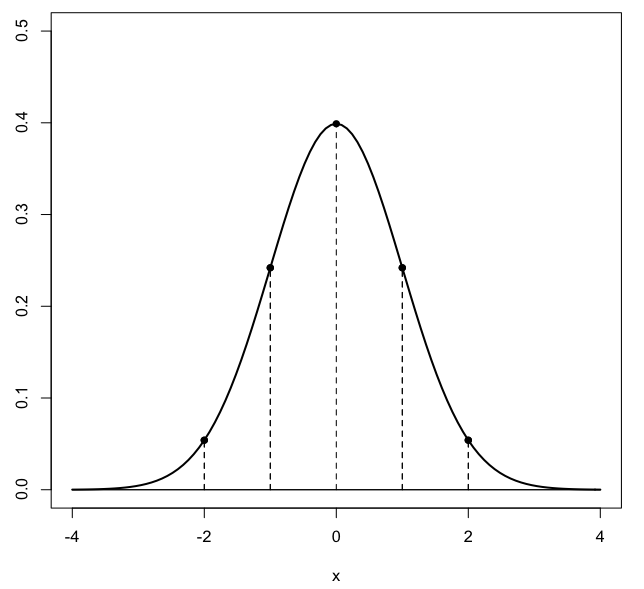
\includegraphics [scale=0.4] {gauss3.png} \end{center}

%break
\title{Optimization problems}
\date{}

\begin{document}
\maketitle
\Large

A general optimization problem expresses some dependence as a function, e.g. $A=f(x)$, where $f(x)$ is moderately complicated.  We wish to find the value of $x$ that gives a maximum (or a minimum) for $A$, perhaps within some limited domain of $x$, or sometimes over all  possible values of $x$.

Usually, the first part is to construct the function $f(x)$, using some constraint that is given in the problem statement.  Then, the basic method is to find the first derivative $A'$ and set it equal to zero, and solve for $x$.

There is no shortage of fun (and challenging) problems of this type.  We did the rectangular area problem earlier in the chapter on higher derivatives.

In this chapter we do problems involving area or volume.  The next chapter has some additional examples.

\subsection*{Three-sided fence}

We wish to build a fence, using an existing barn for one of the sides, so we need fencing only on three sides.  The total length of available fencing is 500 ft.  This is the constraint.

\begin{center} 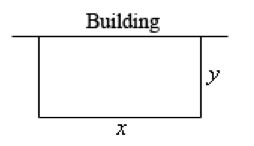
\includegraphics [scale=0.6] {opt1.png} \end{center}

The hard way to solve this is to use the constraint to express $y$ in terms of $x$:
\[ 500 = 2 y + x \]
\[ y = \frac{500 - x}{2} \]
Now write the area as
\[ A = xy = 250x - \frac{1}{2}x^2 \]
Take the first derivative and set it equal to zero:
\[ A' = 250 - x = 0 \]
Clearly, $x=250$ and $y=125$.

The easy way (Nahin) is to imagine that we enclose \emph{another} identical rectangular area on the other side of the barn.  From the first problem it is known that the two areas together should form a square.  Hence, we obtain the half-square as the answer.

\subsection*{Box with an expensive top}

We wish to build a box.  The box is unusual in that the cost of the top and bottom is more than the sides ($10$ v. $6$ per unit area --- let's say it is in square feet but that doesn't really matter).

\begin{center} 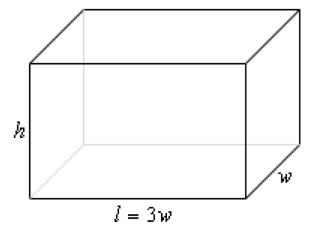
\includegraphics [scale=0.6] {opt2.png} \end{center}

As noted in the figure, the length of the side is three times the width.  We wish to minimize the cost.  

The constraint is that the total volume of the box is $50$ cubic feet.  Using the constraint, we can solve for $h$ in terms of $w$

\[ 50 = 3wwh \]
\[ h = \frac{50}{3w^2} \]

The cost $C$ is
\[ C = 2 \ [ \ 10 \cdot 3w^2 + 6 \cdot wh + 6 \cdot 3 wh \  ] \]
\[ = 2 \ [ 30w^2 + 24wh \  ] \]
\[ = 60w^2 + \frac{800}{w} \]

Take the first derivative and set it equal to zero:
\[ C' = 120 w - \frac{800}{w^2} = 0 \]
\[ w^3 = \frac{800}{120} \]
\[ w = (\frac{800}{120})^{1/3} = 1.88 \]

\subsection*{Box with maximum volume}

This problem features a box with a square base and a total surface area of $S$.  We wish to maximize the volume of the box.

The constraint is the surface area (plus the fact of the square base).  If $b$ is the base length and $h$ is the height, we have that

\[ S = 2b^2 + 4bh \]
\[ h = \frac{S-2b^2}{4b} \]

The volume is
\[ V = b^2 h \]
\[ = b^2 \ \frac{S-2b^2}{4b} \]
\[ = \frac{S}{4} b - \frac{1}{2} b^3 \]

Take the first derivative and set it equal to zero:
\[ V' = \frac{S}{4} - \frac{3}{2}b^2 = 0 \]
\[ S = 6b^2 \]
\[ b = \sqrt{\frac{S}{6}} \]

We can also find $h$
\[ S = 2b^2 + 4bh \]
\[ S = 2\frac{S}{6} + 4h \sqrt{\frac{S}{6}} \]
\[ \frac{1}{3} S = 2h  \sqrt{\frac{S}{6}} \]
\[ h = \frac{1}{\sqrt{6}} \sqrt{S} = b \]

Since $b=h$, what we have is a cube.  Not that surprising. 

\subsection*{Cylindrical can with maximum volume for its surface area}
A cylindrical can is to be formed with a volume of $1.5$ cubic liters.  What are the dimensions if we wish to minimize the surface area (materials used for construction)?

Suppose that the radius is $r$ and the height is $h$.  The formula for volume tells us that
\[ V = 1.5 = \pi r^2 h \]
(Note:  the linear dimensions of this volume, and of $r$,  are in tenths of a meter, since a liter is a cubic decimeter---one-tenth of a meter).

The surface area is 
\[ A = 2 \pi r^2 + 2 \pi r h \]

Substituting for $h$
\[ A = 2 \pi r^2 + 2 \pi r (\frac{1.5}{\pi r^2}) \] 
\[ = 2 \pi r^2 + \frac{3}{r} \] 

Take the first derivative and set equal to zero:

\[ A' = 4 \pi r - \frac{3}{r^2} = 0 \]
\[ r^3 = \frac{3}{4 \pi} \]
\[ r = (\frac{3}{4 \pi})^{1/3} = 0.620 \]
\[ h = \frac{1.5}{\pi r^2}  = 1.24 \]

Multiply by $10$ to get the $r$ and $h$ in centimeters.
\[ r= 6.2 \ \text{cm} \]
\[ h = 12.4 \ \text{cm}  \]

It's no accident that $h = 2r$.

\subsection*{Fancy window}

We wish to construct this window, with a semi-circular arch added on top of the rectangular region below.

\begin{center} 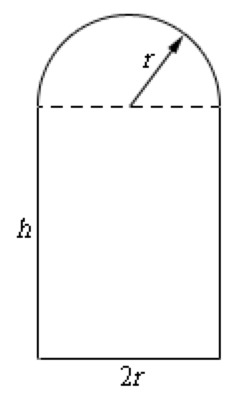
\includegraphics [scale=0.4] {window.png} \end{center}

The quantity to maximize is the area of the window.  The amount of framing for the window is the constraint, with a total length equal to $12$.  Strangely, the framing does not include the dotted line.  Using the constraint, we can solve for $h$ in terms of $r$:
\[ 2h + 2r + \pi r = 12 \]
\[ h = \frac{12 - (2 + \pi) r}{2} \]

The area is 
\[ A = 2rh + \frac{1}{2}\pi r^2 \]
\[ = 12r - (2 + \pi)r^2 + \frac{1}{2} \pi r^2 \]
\[ = 12r - 2r^2 - \frac{1}{2} \pi r^2 \]

We take the first derivative and set it equal to zero:
\[ A' = 12 - 4r - \pi r = 0 \]
\[ r = \frac{12}{4 + \pi} = 1.68 \]
\[ h = \frac{12 - (2 + \pi) r}{2} = 1.68 \]

That's an interesting result!  We should probably revise our drawing, and the client should probably think of a different kind of window.

\subsection*{Rectangle in a circle}

Suppose we have a circle of fixed radius $R$, centered at the origin.  Pick a value for $x$ such that $0 \le x \le R$.  Form the rectangle with all four vertices on the circle.  That is, for the $y$ value corresponding to that $x$, the vertices are $\pm \ x, \pm \ y $.

\begin{center} 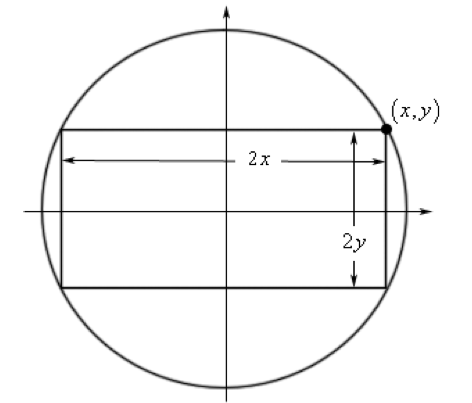
\includegraphics [scale=0.6] {opt3.png} \end{center}

What this means is that given a particular  $x$
\[ y = \sqrt{R^2 - x^2} \]

and therefore the sides of the rectangle are $2x$ and $2\sqrt{R^2 - x^2}$, with area
\[ A = xy = 4x\sqrt{R^2 - x^2} \]

We wish to find the value of $x$ which gives the maximum area.  We will take the first derivative and set it equal to zero.  But, to begin with
\[ \frac{d}{dx} \ \sqrt{R^2 - x^2} = -\frac{1}{2} \frac{2x}{\sqrt{R^2 - x^2}} \]
\[ = -\frac{x}{\sqrt{R^2 - x^2}} \]

so, using the product rule:
\[ A' = (4x)(-\frac{x}{\sqrt{R^2 - x^2}} ) + 4(\sqrt{R^2 - x^2}) = 0 \]
\[ = -\frac{x^2}{\sqrt{R^2 - x^2}} + \sqrt{R^2 - x^2} = 0 \]
\[ x^2 = R^2 - x^2 \]
and since $x^2 + y^2 = R^2$

\[ x^2 = x^2 + y^2 - x^2 = y^2 \]
Thus, $x=y$.  So the maximum area is for a square.  No longer a surprise, I trust.

\subsection*{Mrs. Sidway's problem}

This actually a volume problem, but whatever.

In Acheson we find a problem published in a 1714 edition of \emph{The Ladies Diary: or The Woman's Almanack}, posed by a Mrs. Sidway (as a gardening problem, no less).

\begin{center} 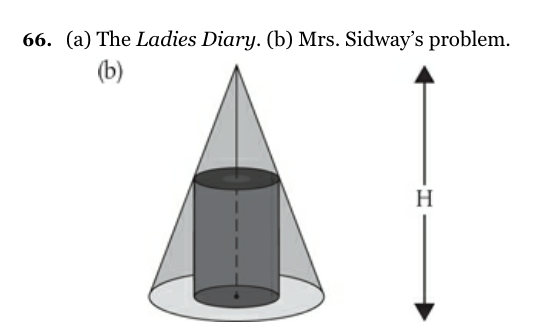
\includegraphics [scale=0.6] {sidway.png} \end{center}

If a cylinder lies contained within a cone (with its upper edge lying along the surface of the cone), how large should the radius be in order for the cone to have the maximum volume?

I find it easier to think about this problem by first placing the origin at the left of the figure, before moving it to the center for the second part.

The cone has fixed height $H$ and radius $R$.  If we place the origin at the left edge and allow a variable $x$ to range from this origin to the right up to a distance $R$, you should be able to see first, that for any $x$
 
\[ \frac{h}{x} = \frac{H}{R} \]

by similar triangles.  This is a standard relationship for the cone.

But the radius of the cylinder, measured from the central axis of both cylinder and cone is

\[ r = R - x = R - h \frac{R}{H} \]

Rearranging

\[ h = \frac{H}{R} (R - r) \]

At this point, we compute the volume as

\[ V = Ah = 2 \pi r^2 \cdot \frac{H}{R} (R - r) \]

$V$ depends on $r$ and we can take the derivative with respect to $r$ and then set it equal to zero in order to find the maximum.  

When we do this, the constants ($2 \pi$) will carry through into the first derivative and then disappear since we set the result equal to zero.  Thus, we can ignore them

\[ V \approx r^2 \cdot \frac{H}{R} (R - r) \]
\[ = r^2 \cdot (H - \frac{H}{R} r) \]
\[ = Hr^2 - \frac{H}{R} r^3 \]

The derivative is

\[ 0 = 2Hr - 3 \frac{H}{R} r^2 \]
\[ 2r = 3 \frac{r^2}{R} \]
\[ \frac{2}{3} R = r \]

The maximum volume is obtained with $r$ equal to two-thirds the radius of the cone at the bottom.


\end{document}  